\documentclass[a4paper,11pt,italian]{report}
\usepackage[italian]{babel}
\usepackage{fullpage}
\usepackage{graphicx}
\usepackage{latexsym}
\usepackage{gensymb}
\usepackage{multirow}
\usepackage{amsmath,amssymb,amsfonts}
\usepackage[infoshow,debugshow]{tabularx}
\usepackage[T1]{fontenc} 
\usepackage[utf8]{inputenc} 
\usepackage[italian]{varioref}
\usepackage[infoshow,debugshow]{tabularx}
\usepackage{booktabs,caption}
\usepackage{lipsum}
\usepackage{url}
\usepackage{caption}
\usepackage[figuresright]{rotating}
\usepackage[autostyle,italian=guillemets]{csquotes}
\usepackage{cite}
\usepackage{float}
\usepackage{setspace}
\usepackage{threeparttable}
\usepackage{siunitx}

\DeclareGraphicsExtensions{.pdf}

\begin{document}

\author{Riccardo Antonelli, Federico Chiossi, Patato Schiavi}
\title{Timing}

\maketitle

\section{Obiettivi}

% misura andamento del guadagno dei PMT in funzione della tensione applicata determinando il punto di lavoro ottimale
% determinare la calibrazione in energia degli scint organici e la ris energetica dell'analisi dei Compton edge
% determinare ritardo esterno CFTD che ottimizza la ris t del sistema
% determinare andamento ris temporale in f del range dinamico dei segnali analizzati dal CFTD

\begin{itemize}

\item Misura dell'andamento del guadagno dei PMT in funzione della tensione applicata e determinazione del punto di lavoro ottimale
\item determinazione della calibrazione in energia degli scintillatori organici e la risoluzione energetica dell'analisi dei Compton edge
\item determinazione del ritardo esterno CFTD che ottimizza la risoluzione temporale del sistema
\item determinazione dell'andamento della risoluzione temporale in funzione del range dinamico dei segnali analizzati dal CFTD

\end{itemize}

\section*{Fit del profilo Compton}

Per la calibrazione dei rivelatori in energia dei raggi X e in risoluzione energetica forniamo i risultati di due metodi: il primo (\textbf{SEMIGAUSS}), basato su i risultati di una simulazione Monte-Carlo fatta dal professor Viesti, che utilizza i valori di un fit Gaussiano sui due profili Compton troncati. Il secondo (metodo \textbf{FIT}) è un modello semi-empirico da noi sviluppato basato su un fit esplicito di un profilo Compton.\\

Come profilo energetico "grezzo" (senza considerare la risoluzione dell'apparato) consideriamo la distribuzione di Klein-Nishina integrata. Definiamo $\text{edge}_{1,2} \approx \SI{340}{\kilo\electronvolt}, \SI{1062}{\kilo\electronvolt}$ gli edge Compton per i fotoni rispettivamente a $511$ e $\SI{1275}{\kilo\electronvolt}$. Se $c$ è il canale, e $(y,e_1,e_2,k)$ sono parametri che descrivono la distribuzione, definiamo $E_0$ la stima dell'energia al canale $0$:

\[E_0 := \left(\text{edge}_1 - \frac{e_1}{e_2} \, \text{edge}_2\right)/\left(1-\frac{e_1}{e_2}\right) \]

I parametri $e_i$ sono le posizioni in canali dei due Compton edge. Sia

\[E(c) := E_0 + \left(\frac{\text{edge}_1 - E}{e_1}\right) c\]

la stima dell'energia al canale $c$. Notare che abbiamo semplicemente effettuato la calibrazione tale per cui $E(e_i) = \text{edge}_i$.\\

A questo punto definiamo la distribuzione

\[ A(c) := y \sum_i k_i \left( 2-2 \frac {E} {\epsilon_i - E} + \frac{E^2}{(\epsilon_i-E)^2} + \frac{E^2}{\epsilon_i (\epsilon_i-E)} \right) \chi(c<e_i) \]

La somma è sui due picchi Compton; $k_1 = 1$ e $k_2 = k$, parametro che racchiude il rapporto in ampiezza fra i due picchi Compton. $y$ è un fattore di scala globale sulle frequenze. $\epsilon_i$ sono le energie dei fotoni, $\sim 1275$ e $\SI{511}{\kilo\electronvolt}$. $\chi$ è una funzione indicatrice che tronca il profilo in corrispondenza del picco Compton.\\

Per tenere conto della risoluzione dello strumento effetuiamo una convoluzione del profilo $A(c)$ con una gaussiana di integrale unitario. Questa nuova distribuzione ha un parametro addizionale, la deviazione standard della gaussiana $\sigma$:

\[ B(c;y,e_1,e_2,k,\sigma) = A(c;y,e_1,e_2,k) * \text{gauss}(c';\sigma) \]

Tuttavia questo modello non fitta bene i dati. Vogliamo qui suggerire un modello che trova un migliore riscontro coi dati sperimentali. Supponiamo che la FWHM generato da un fascio di raggi X di fissata energia sia proporzionale all'energia stessa del fascio, ovvero che la $\sigma$ sia una funzione lineare del canale:

\[ \sigma(c) = \gamma c \]

Con $\gamma$ un parametro adimensionale. Per cui la distribuzione risultante è

\[ B(c; y, e_1, e_2, k ,\gamma) = A(c;y,e_1,e_2,k) * \text{gauss}(c';\gamma c) \]

(la scrittura è formale, dal momento che non si tratta più di una convoluzione vera e propria.) Nel dettaglio il calcolo effettuato è stato

\[ B(c) = \sum_j A(c+j)\,  \text{gauss}(j;\gamma c) \]

con un range ragionevole per $j$.\\

La distribuzione finale è fittata ai dati mediante un metodo a forza bruta; lo spazio dei parametri è diviso in celle e queste sono esplorate per trovare il set che minimizza lo scarto quadratico totale. Si ripete la ricerca raffinando la griglia. Lo svantaggio di questo metodo è il costo computazionale: per avere tempi di esecuzione nell'ordine di alcuni minuti è necessario fornire al programma un range non eccessivo in cui far variare i parametri. 

Un tipico esempio dell'utilizzo del programma è mostrato di sequito.
(Mettere immagine)
Si noti che il fit riesce ad approssimare bene anche il compton edge a 1275 keV. Per dare una stima dell'errore sui valori ottenuti in grafico è anche mostrato il fit in cui il parametro $\sigma$ (o compton edge) è stato incrementato (o diminuito) di un 20\% (forse 30\%?) dal valore ottimale.
\section{Analisi}

\subsection*{Guadagno - Voltaggio}

Vogliamo studiare il comportamento dei PMT in funzione della differenza di potenziale dei dinodi. Chiaramente aumentando il voltaggio aumenta il guadagno, ma per i limiti dell'elettronica (dell'ADC in particolare) per i voltaggi di 1800 e 1900 V è necessario ridurre il guadagno dell'amplificatore da x100 a x40. Il risultato è che il valore ottimale di lavoro è di 1700 V. 

Dal parametro $\sigma/C$ (Rapporto adimensionale tra il centro e la $\sigma$ del fit gaussiano eseguito in un interno del compton edge) si ha una stima della risoluzione dell'apparato. Osserviamo dalle figure di seguito che tale parametro rimane pressochè lo stesso col variare del voltaggio.
L'errore è stato ottenuto per propagazione tenendo conto della covarianza dei due valori.


\begin{minipage}{\linewidth}
\begin{minipage}{0.45\linewidth}
\centering
\begin{figure}[H]
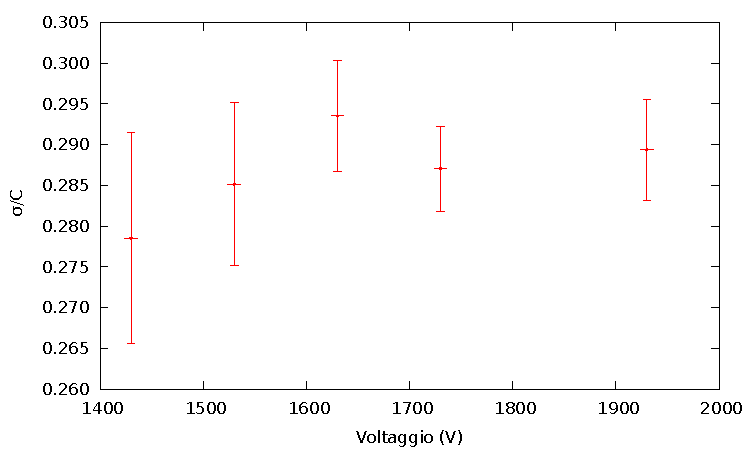
\includegraphics[width=\columnwidth,keepaspectratio]{../out/chio/Guadagno_R1}
\caption{\small{Andamento della risoluzione energetica in funzione del voltaggio per il rivelatore 1}}
\end{figure}
\end{minipage}
\hspace{\fill}
\begin{minipage}{0.45\linewidth}
\centering
\begin{figure}[H]
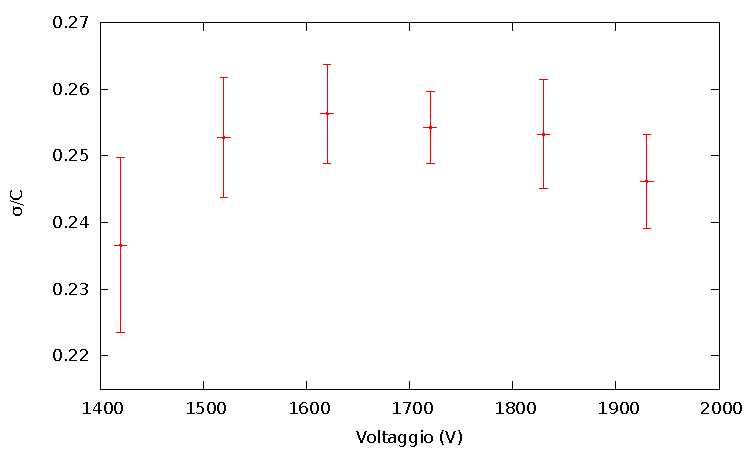
\includegraphics[width=\columnwidth,keepaspectratio]{../out/chio/Guadagno_R2}
\caption{\small{Andamento della risoluzione energetica in funzione del voltaggio per il rivelatore 2}}
\end{figure}
\end{minipage}
\end{minipage}

Usando il metodo (FIT) si trovano risultati analoghi.

\subsection*{Risoluzione energetica}

\subsubsection*{Metodo \textbf{SEMIGAUSS}} 
Calcoliamo il parametro $\sigma/C$ per il voltaggio di circa 1730 V per il rivelatore 1 e 2 sia per il compton edge dei fotoni di 511 keV e che per quello di 1275 keV. Dai grafici sulle dispense fatti da viesti posssiamo stimare qialitativamente la risoluzione energetica e lo shift dal centroide misurato al vero valore del compton edge. Introduciamo per la calibrazione i parametri $m,q$ secondo $\text{energia} = m \;\text{canali}+ q$.

\begin{table}[!hp]
\caption{\small{Calibrazione in energia per i rivelatori}}
\centering
\begin{threeparttable}[b]
{
$
\begin{array}{cccc}
\toprule
$Energia fotone (keV)$ & \sigma/C & $Risoluzione energetica (keV)$ & $Shift (keV)$\\
\midrule
511$ R1$ & 0.287 \pm 0.005 & 50-65 &  60-85     \\
1275 $ R1$ & 0.219 \pm 0.013 & 35-50 &  40-80      \\
511$ R2$ & 0.254 \pm 0.006 &  45-60 &  50-75      \\
1275 $ R2$ &  0.255 \pm 0.030 &  40-60 & 50-100       \\ 	 
\bottomrule
\end{array}
$
}
\end{threeparttable}
\label{tab:parametrisemigauss}
\end{table}

\subsubsection*{Metodo \textbf{FIT}}

\begin{table}[!hp]
\caption{\small{Calibrazione in energia per i rivelatori}}
\centering
\begin{threeparttable}[b]
{
$
\begin{array}{ccccc}
\toprule
$Rivelatore$ & \sigma/C & $Risoluzione a $\SI{511}{keV} & m & q  \\
\midrule
R1 & 0.15 & \SI{76}{keV} & \SI{1.45}{keV}/\text{canale} & \SI{140.8}{keV} \\ 
R2 & 0.14 & \SI{72}{keV} & \SI{1.72}{keV}/\text{canale} & \SI{119.2}{keV} \\
\bottomrule
\end{array}
$
}
\end{threeparttable}
\label{tab:parametrifit}
\end{table}

%ch1
%
%256.093 e1
%782.222 e2
%
%0.147942 gamma
%
%1.45 m
%
%140.8 q
%
%ch2
%
%229.21 e1
%672 e2
%
%1.72 m
%
%119.16 q
%
%0.135861 gamma


\subsection*{Risoluzione temporale}

Vogliamo determinare il ritardo che ottimizza la risoluzione temporale dell'apparato.\\

La calibrazione temporale è stata effettuata acquisendo lo spettro temporale del TAC variando il delay utilizzando ritardi predefiniti. Dopodiché fittiamo una gaussiana su ogni spettro; infine fittiamo il ritardo noto con i centroidi ottenuti:


Risulta $t = (0.0247 \pm 0.0002)\, \si{\nano\second}\,\mathrm{canali}^{-1} \cdot C + (0.53 \pm 0.16 \, \si{\nano\second})$.\\

\begin{minipage}{\linewidth}
\begin{minipage}{0.45\linewidth}
\centering
\begin{figure}[H]
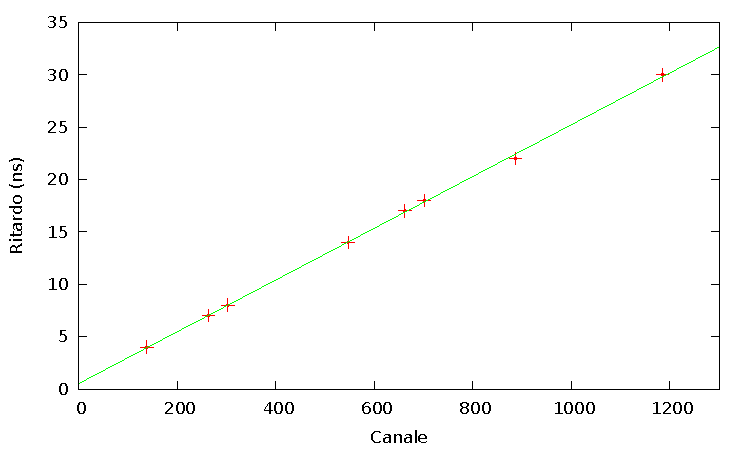
\includegraphics[width=\columnwidth,keepaspectratio]{../out/chio/Cal_DnDt}
\caption{\small{Calibrazione tempo-canale}}
\end{figure}
\end{minipage}
\hspace{\fill}
\begin{minipage}{0.45\linewidth}
\centering
\begin{figure}[H]
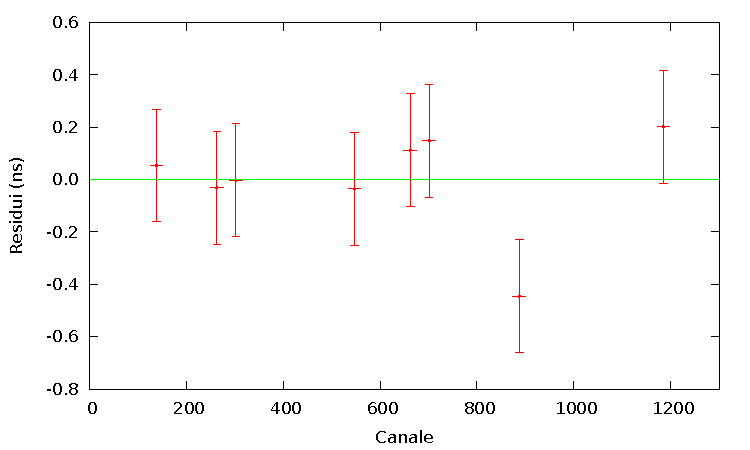
\includegraphics[width=\columnwidth,keepaspectratio]{../out/chio/Residui_cal_DnDt}
\caption{\small{Residui della cal. tempo-canale}}
\end{figure}
\end{minipage}
\end{minipage}

\begin{table}[!hp]
\caption{\small{Dati della calibrazione tempo-canale}}
\centering
\begin{threeparttable}[b]
{
$
\begin{array}{cccc}
\toprule
 $Ritardo (ns)$ & $Centroide$ & \sqrt{\chi^2/\text{ndf}} & $Residui$ \\
\midrule
4&	138.20	&	0.22&	0.06\\
7&	263.09	&	0.22&	-0.03\\
8&	302.41	&	0.22&	0.00\\
14&	546.71  &       0.22&   -0.03\\
17&	662.20	&	0.22&	0.11\\
18&	701.20	&	0.22&	0.15 \\
22 &	887.17	&	0.22&	-0.44\\
30&	1184.93	&	0.22&	0.20\\
\bottomrule
\end{array}
$
}
\end{threeparttable}
\label{tab:Cal_DnDt}
\end{table}

\`E necessario stimare inoltre il ritardo corrispondente ai cavi LEMO. Fittiamo il ritardo misurato con la lunghezza totale di LEMO:

\begin{minipage}{\linewidth}
\begin{minipage}{0.45\linewidth}
\centering
\begin{figure}[H]
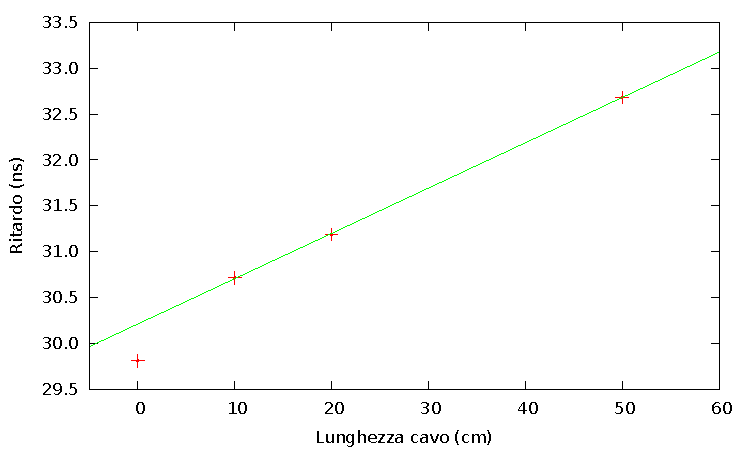
\includegraphics[width=\columnwidth,keepaspectratio]{../out/chio/tempo_residui}
\caption{\small{Stima ritardo per lunghezza dei cavi LEMO}}
\end{figure}
\end{minipage}
\hspace{\fill}
\begin{minipage}{0.45\linewidth}
\centering
\begin{figure}[H]
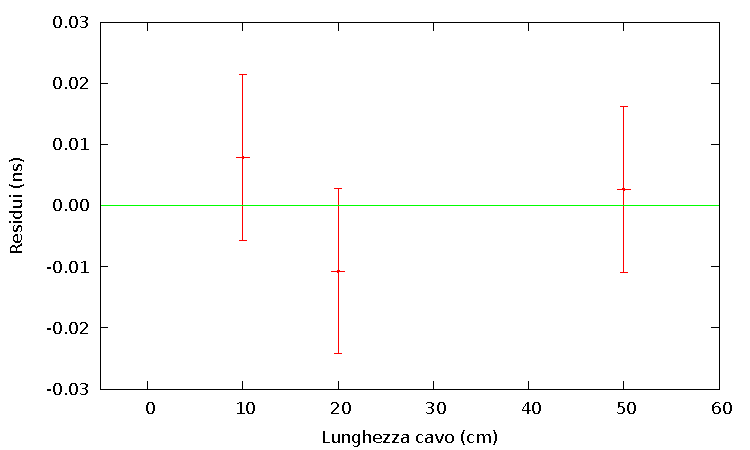
\includegraphics[width=\columnwidth,keepaspectratio]{../out/chio/tempo_ritardores}
\caption{\small{Residui ritardo per lunghezza dei cavi LEMO}}
\end{figure}
\end{minipage}
\end{minipage}

\begin{table}[!hp]
\caption{\small{Dati della calibrazione tempo-canale}}
\centering
\begin{threeparttable}[b]
{
$
\begin{array}{ccccc}
\toprule
 $Lunghezza (cm) $ & $Centroide$ & $Ritardo (ns) $  & $Residui$  &\sqrt{\chi^2/\text{ndf}} \\
\midrule
0&	1185.23 &       	29.806   &	-	&	0.014\\
10&	1221.91 &		30.712   &	0.008	&	0.014\\
20&	1241.16	&		31.188	&	-0.010&	0.014\\	
50&	1301.71	&		32.683 &      0.003	&0.014\\
\bottomrule
\end{array}
$
}
\end{threeparttable}
\label{tab:tempo_ritardo}
\end{table}
Dal fit lineare risulta: ritardo (ns) $= 0.0494 \pm 0.0005 (ns/cm) \cdot \text{Lunghezza (cm)} + (30.211 \pm 0.015 ns)$ . In buon occordo con il dato teorico di 0.05 ns/cm. Rispetto al ritardo predefinito (30 ns) si sono aggiunti tramite una I, cavi da 10, 20 e 50 cm. Possiamo stimare il ritardo dovuto alla I estrapolando dal fit il ritardo a 0 cm e sottraendo il ritardo predefinito ottenendo $ 0.405 \pm 0.013 $ ns.

\section{Conclusioni}

\end{document}
